\documentclass{article}
\usepackage{graphicx} %For importing images
\usepackage[labelfont=bf]{caption} %For making "Figure i:" label bold
\usepackage{enumerate}
\usepackage{hyperref}
\begin{document}

  \title{White Paper: How Artificial Intelligence Affects the Work Force}
  \author{Michael Giancola - WR 1011}
  \date{\today}
  \maketitle

  \cleardoublepage

  \section{Introduction}
    \paragraph{}
      The McKinsey Global Institute identified seven emerging technologies which
      they expect will have a one trillion dollar or greater impact on the economy.$_{[1]}$
      One of the seven was ``Advanced Robotics''; or in other words, artificially
      intelligent machines. The technologies, including robotics, are advancing
      so quickly that it is difficult for companies to keep up. Employees in virtually
      every field will have to plan ahead so they can best adapt with changing technology.
      With the economic impact that McKinsey predicted, AI could significantly
      stimulate the world economy - whether the change is good or bad depends
      on how well executives prepare their companies for the changing circumstances.

    \paragraph{}
      While I wouldn’t call current day AI ``intelligent'', it plays a unique
      role in the workforce. In particular, a large subset of these machines are used
      for automating mundane, repetitive tasks - like checking in at the airport
      before a flight. These machines don’t require much real intelligence,
      because all they have to do is request some data from a user, provide means
      of inputting that data, and finally pass the information along to where it
      needs to go.

    \paragraph{}
      With the advent of true AI, much more sophisticated work will be able to
      be automated by machines. A truly intelligent machine would be able to
      replace most knowledge workers. That is, people whose job it is to think.
      This includes academics, engineers, insurance underwriters, and many more.
      While current day automation affects a low echelon of work, true AI could
      rock the middle class job market, causing a large sector of the working
      class to lose their jobs.

    \paragraph{}
      As is usually the case with emerging technology, corporate executives have
      two options: resist, or adapt. In this scenario, it seems advantageous for
      everyone involved to adapt. True AI is inevitable, and any company that
      refuses to adapt to the changing circumstances will be unable to compete
      in their market. Furthermore, if our society plans ahead, and determines
      how to best coexist with intelligent machines, it could increase our
      productivity exponentially.

  \section{Types of Intelligence}

    \paragraph{}
      With the many different examples of AI in society today, like airport kiosks,
      Siri, and Google's autonomous car, it is difficult to define exactly what
      artificial intelligence is. However, in my opinion, we can categorize them
      into three distinct groups. The first is ``dumb''
      intelligence; these machines automate a simple task, usually by requesting
      data from a user and performing a task based on that data. A simple example
      is a airport kiosks used to check in before a flight. They are not intelligent at all,
      they just follow a simple computer program. However, they are well known
      and relevant to the discussion of AI.

    \paragraph{}
      The second is ``simulated'' intelligence;
      these machines analyze the data that they receive in a way that makes them
      appear intelligent.
      For example, a GPS can find a route between two points, and even figure out what
      to do if there's a detour along the path. However, in reality it is just a
      simple algorithm processing a relatively small amount of data.

    \paragraph{}
      For a machine to possess ``true'' intelligence, it should be able to perform some action,
      assess the consequences of its action, and, ultimately, learn from its
      successes and failures. This isn't a hard definition; I think that
      AI will continue to adapt, and so will our definition of intelligence.

    \paragraph{}
      Figure 1 shows what surveyed executives believe constitutes artificial
      intelligence. Like almost one third of people surveyed, I believe that
      artificial intelligence is a combination of the things listed. The ability
      to learn and adapt is, to me, the hallmark of AI. However for AI to feel
      ``real'' to most people, it must be able to communicate with them in a
      reasonable manner. My prediction is that all of these components will come
      together in the next few decades as artificial intelligence continues to
      advance.\\

      \begin{figure}[ht]
        \centering
        \captionsetup{width=.85\linewidth}
        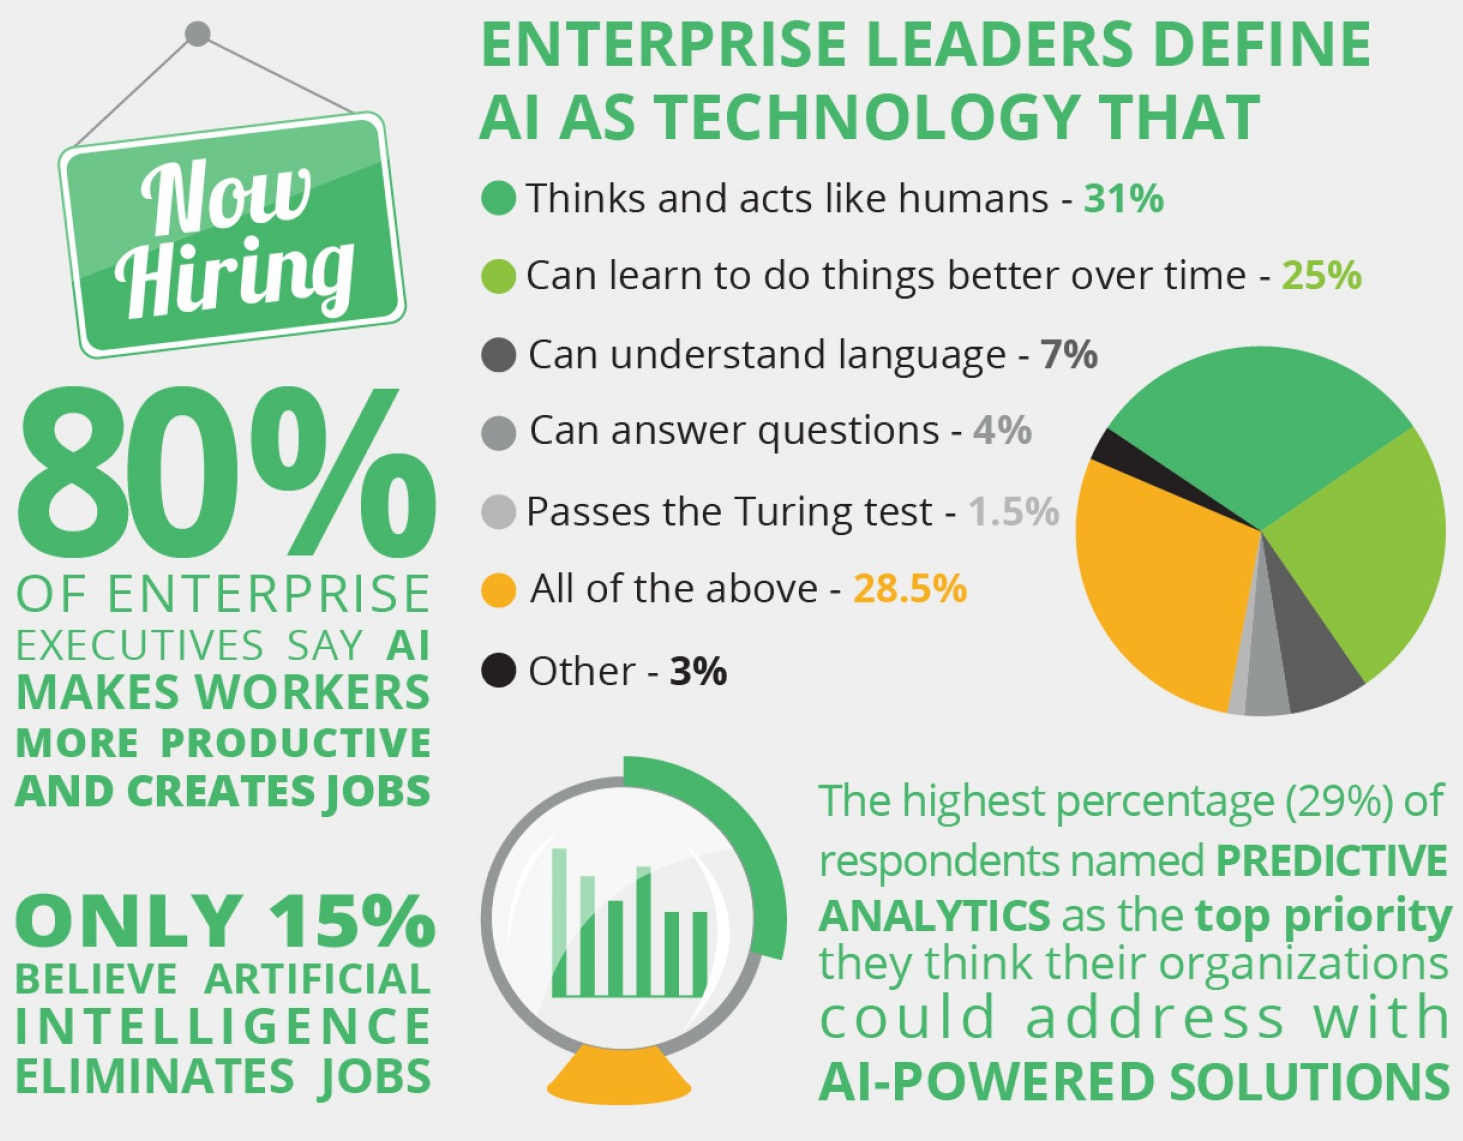
\includegraphics[width=0.85\textwidth,height=\textheight, keepaspectratio]{Figure1}
        \caption{Enterprise leaders are surveyed on their perceptions of AI in the workforce.
                 \href{http://thumbnails-visually.netdna-ssl.com/artificial-intelligence-is-not-killing-jobs_557b4376e27b8_w1500.jpg}
                 {\textbf{Source}}}
      \end{figure}

  \cleardoublepage

  \section{Current Effects}
    \paragraph{}
      Another interesting statistic from the survey cited in the figure above is
      that ``only 15\% [of people surveyed] believe that AI eliminates jobs''.$_{[2]}$
      This statistic really surprised me, as it seems to counter popular opinion
      - just see how many articles come up from Google searching ``Artificial Intelligence
      Destroys Jobs''. However, this particular study from \textit{NarrativeScience}
      found that AI may actually play a very positive role in the workplace. In
      fact, \\

      \begin{center}
        \fbox{
          \parbox{0.75\textwidth}{
          ``...many executives are learning that AI-powered solutions can step in
          to solve the data-use and comprehension problem, provide a competitive
          advantage, free their employees to focus on strategic initiatives and even
          create jobs.''$_{[2]}$
          }
        }
      \end{center}

    \paragraph{}
      While this outlook is nice, other studies still believe that AI has
      the potential to hurt the job market. Figure 2 compares
      the labor productivity in the US to the relative
      level of private employment. There is a strong correlation between them
      until the early 2000s, where the trend stops. Many economists, including
      Erik Brynjolfsson, believe this could be cause for concern.
      In an interview with TechRepublic, Brynjolfsson
      commented on this trend:

      \begin{figure}[h]
        \centering
        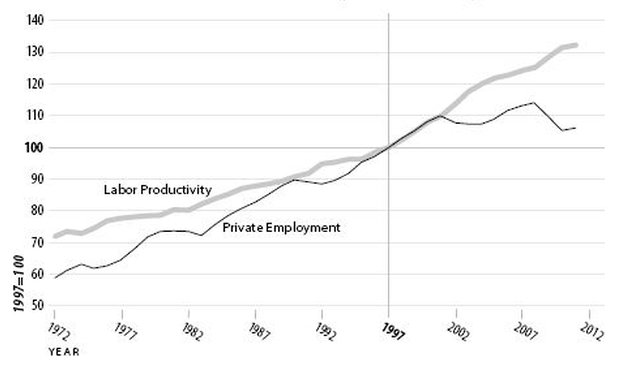
\includegraphics[width=\textwidth,height=\textheight, keepaspectratio]{Figure2}
        \caption{Labor Productivity vs. Private Employment.
                 \href{http://www.techrepublic.com/article/ai-is-destroying-more-jobs-than-it-creates-what-it-means-and-how-we-can-stop-it/}
                 {\textbf{Source}}}
      \end{figure}

      \begin{center}
        \fbox{
          \parbox{0.75\textwidth}{
          ``Unlike much of the 20th century, we're now
          seeing a falling ratio of employment to population ...[we think] that
          many of the underlying trends in technology are likely to accelerate this
          so it’s something we need to pay some serious attention to.''$_{[3]}$
          }
        }
      \end{center}

    \paragraph{}
      While it is true that this is a serious concern that we must attend to,
      there was a lot of technological advancement in the late 90’s through
      the early 2000s. Therefore, it is near impossible to claim that AI was
      the sole cause for the disparity between labor productivity and private
      employment. Indeed, it is difficult to single out the effects of AI,
      especially because it is such a new development. As such, I believe that
      the results of the \textit{NarrativeScience} study should be more closely
      considered. Companies which utilize AI will have an advantage
      over their competitors who do not.

  \section{Collaboration of Man and Machine}

    \paragraph{}
      Now, onto the important question that this paper attempts to answer.
      If companies are to improve their productivity by introducing intelligent
      machines to the workplace, how can these machines
       and humans best collaborate? More importantly, what will be the place
      of humans in the workforce, with robots doing a lot of the work that humans
      do now?

      \begin{figure}[h]
        \centering
        \captionsetup{width=.85\linewidth}
        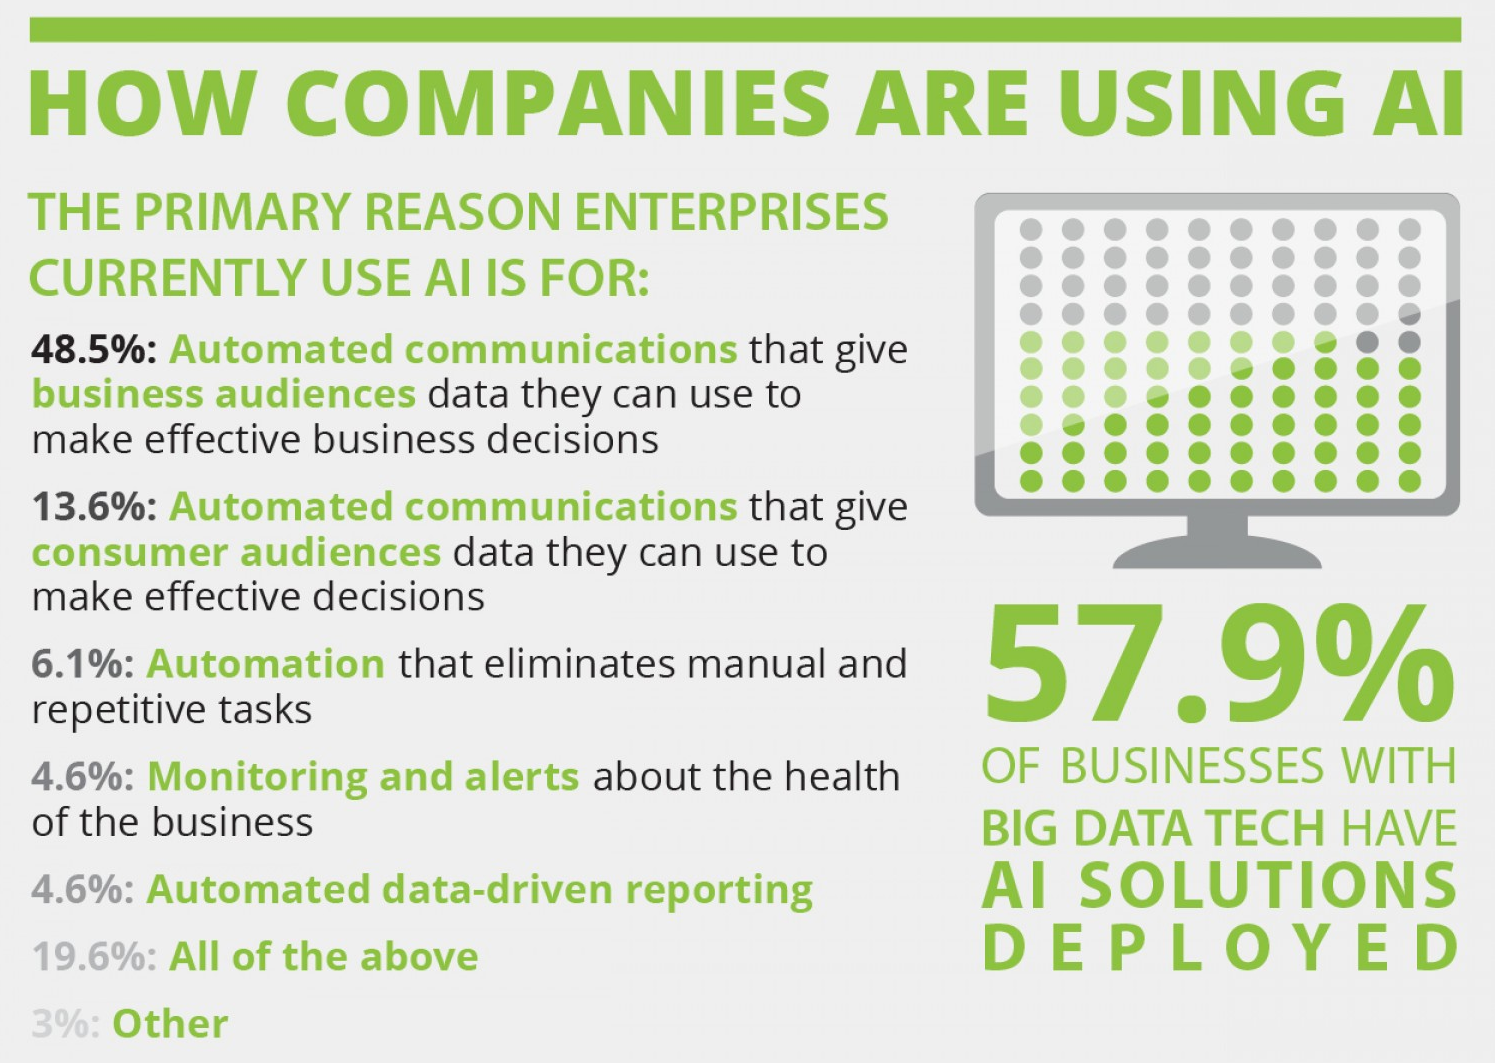
\includegraphics[width=0.85\textwidth,height=\textheight, keepaspectratio]{Figure3}
        \caption{Over 90\% of companies surveyed currently use some form of AI for automation.
                 \href{http://thumbnails-visually.netdna-ssl.com/artificial-intelligence-is-not-killing-jobs_557b4376e27b8_w1500.jpg}
                 {\textbf{Source}}}
      \end{figure}

    \paragraph{}
      Figure 3 highlights another statistic from the \textit{NarrativeScience}
      study referenced earlier. They found that over 90\% of respondents use AI
      primarily for automation. Many repetitive, mundane tasks can easily be
      done by intelligent machines. However, soon they will be able to take over
      more complex tasks.

    \paragraph{}
      Journalists Martin Dewhurst and Paul Willmott of McKinsey \& Company
      speculated that human workers ``...will be able to make the biggest difference
      through the human touch.''$_{[4]}$ In other words, humans will be needed to
      analyze the findings of intelligent machines and make critical
      decisions, like deciding the direction for the future of the company.

    \paragraph{}
      There is also a basic need for “soft skills”, which Dewhurst and Willmott
      believe robots will never attain. At least in the foreseeable future, it
      is difficult to imagine humans willingly taking orders from a robot.
      Similarly, it seems unlikely that a robot leader could inspire the same
      drive into workers as a human leader. Emotion will likely be one of the
      most difficult things for intelligent machines to capture. Even once they
      do, conveying it in a way that is received well by humans is a whole other
      battle. Ultimately, the integration of AI will likely be similar to many
      other technological advances; it will change the way we work, but won't
      replace us.

  \section{Moving Forward}
    \paragraph{}
      Alert the presses, yell from the rooftops, robots are \textit{not} coming
      for your jobs. While it may seem that intelligent machines are going to
      replace us, a machine is as likely to replace the human worker as a printer
      is. Sure, a printer takes the job of a scribe who would have written the
      documents that it now prints. On the other hand, it frees up humans to
      do more important work. I believe this is what intelligent machines will
      do as well.

    \paragraph{}
      Business leaders need to prepare their companies to adapt to
      changing tides, understanding that the role of humanity in the workforce
      is changing. However, humans will always have skills that robots do not.
      Eighty percent of respondents to the \textit{NarrativeScience} study believe
      that ``AI improves worker performance and creates jobs.''$_{[2]}$ If
      executives determine how to integrate AI and human workers in their company,
      there will be a twofold effect. First, it will keep
      most people employed, making money, and contributing to a healthy economy.
      Second, it will make our companies more productive, further stimulating the
      economy.

  \cleardoublepage

  \section{Citations}
    \begin{enumerate}[ {[}1{]} ]
      \item James Manyika, Michael Chui, Jacques Bughin, Richard Dobbs,
            Peter Bisson, and Alex Marrs (May 2013). ``Disruptive technologies:
            Advances that will transform life, business, and the global economy''
            \textit{McKinsey\&Company}.
            \href{http://www.mckinsey.com/insights/business_technology/disruptive_technologies}{\textbf{Link}}
            Last Accessed 2/11/16

      \item NA (2015). ``2015 State of Artificial Intelligence \& Big Data in
            the Enterprise'' \textit{NarrativeScience}.
            \href{https://www.narrativescience.com/filebin/images/Landing_Page/2015_State_of_AI_and_Big_Data_in_the_Enterprise.pdf}
                  {\textbf{Link}} Last Accessed 2/11/16

      \item Heath, Nick (ND). ``Why AI could destroy more jobs than it creates,
            and how to save them'' \textit{TechRepublic}.
            \href{http://www.techrepublic.com/article/ai-is-destroying-more-jobs-than-it-creates-what-it-means-and-how-we-can-stop-it/}
                 {\textbf{Link}} Last Accessed 2/11/16

      \item Martin Dewhurst, Paul Willmott (September 2014). ``Manager and
            machine: The new leadership equation'' \textit{McKinsey\&Company}.
            \href{http://www.mckinsey.com/insights/leading_in_the_21st_century/manager_and_machine}
                 {\textbf{Link}} Last Accessed 2/11/16


    \end{enumerate}

  \end{document}
